\section{Execution}

\subsection*{Rotation Algorithms}

\begin{figure}[ht]
\centering
\caption{Rotation Algorithms UML}
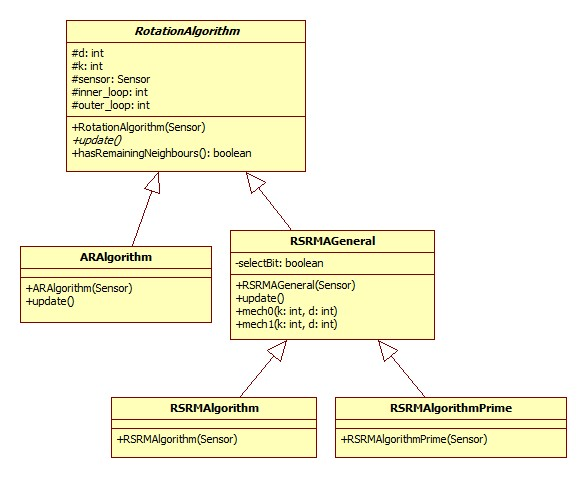
\includegraphics[height = 8cm]{pics/algo.jpg}\\[0.5cm]    
\label{fig:rotalgo}
\end{figure}

To implement the rotation algorithms we have decided to use a strategy pattern, as shown in 
figure \ref{fig:rotalgo}, to allow the MainThread to update a RotationAlgorithm without specifically 
knowing which it is. The main thread includes a List of RotationAlgorithms that get 
initialized, based on GUI parameters, to a more specific algorithm such as ARA, RSRMA, or 
RSRMA' . It was easy to see that a strategy pattern was needed, simply because all the 
algorithms shared a number of things in common. Using the strategy pattern allowed us to 
abstract common methods and variables, such as the delay (d), sectors (k) variables and mech0 
and mech1 methods. This produced more elegant code. Each algorithm takes in a Sensor that it 
will be responsible for rotating, and based on the Sensor that's given it determines the 
algorithm's delay (d) and number of sectors (k).  Because this algorithms do not spawn their 
own threads and rely on the MainThread to loop through them, the delay loops were done slightly 
differently. The update methods for each algorithm are responsible for rotating the Sensor. In 
the update methods the outer\_loop and inner\_loop variables are used to simulate delay. In the 
case of the ARAlgorithm, where the original algorithm is described in the assignment and the 
additional papers, the for loop inside of the while loop acted as a delay. The way that was 
implemented was that the while loop was the MainThread update loop and the inner for-loop was 
represented by the outer\_loop variable, to cause delay. To be more specific the outer\_loop 
variable upon initialization of an ARAlgorithm is set to the Sensor's 'd', it's color/prime. 
Evertime the update happens for the ARAlgorithm the outer\_loop variable decrements, until it 
reaches  zero. When it is zero the Sensor updates, causing a turn, and the outer\_loop variable 
is reinitiated to the Sensor's 'd'. This simulates the delay in the algorithm, and although the 
loop does not look the same, it functions the same way. For the RSRMA and RSRMA' the loops 
where handled in a similar fashion. However each time the outer\_loop variable reached zero, it 
would randomly pick between mech0 and mech1. With the level of abstraction that was made by 
implementing the strategy pattern, the RSRMAGeneral contained majority of how the randomized 
algorithms functioned. It was noticed that the difference between RSRMA and RSRMA' was that one 
passed in 'k' and 'd' to the mechs, while the other passed in two 'k', treating one of the 'k' 
as a 'd'. Thus the only code that RSRMAlgorithm and RSRMAlgorithmPrime possess is one assigns 
the Sensor's 'k' to the algorithm's 'k' and the Sensor's 'd' to the algorithm's 'd' while the 
other assigns the Sensor's 'k' to both the algorithm's 'k' and 'd'.
